\subsection{Numerical Results} \label{ssec: numResult}
Let us compare the $L^2(\Q \otimes \, dt)$ error  
$\lVert Y^{K,\frakF} - Y \rVert^2_{*} $ in the Brownian case for the two avenues discussed at the beginning of this section. When $Y^{K,\frakF} = (f \circ \pi^{K,\frakF})(X) $, the error is calculated using Monte Carlo simulations. As in  \Cref{sec:numResultX}, we choose $T=1$, $N=10^4$ and $K\in \{1,\ldots,128\}$.  
\Cref{fig:L2Error} displays the result for the running maximum, integral and average functionals. We also add the Brownian motion itself, corresponding to the identity functional $f(X)=X$. We observe a clear improvement when projecting the transformed path. Moreover, it comes as no surprise that smooth functionals (integral, average) exhibits a faster rate of convergence than the running maximum, highly sensitive to local behaviours of a path. 

\begin{figure}%[H]
    \centering
    \caption{$L^2(\Q \otimes dt)$ approximation errors. }
    \vspace{-2mm}
    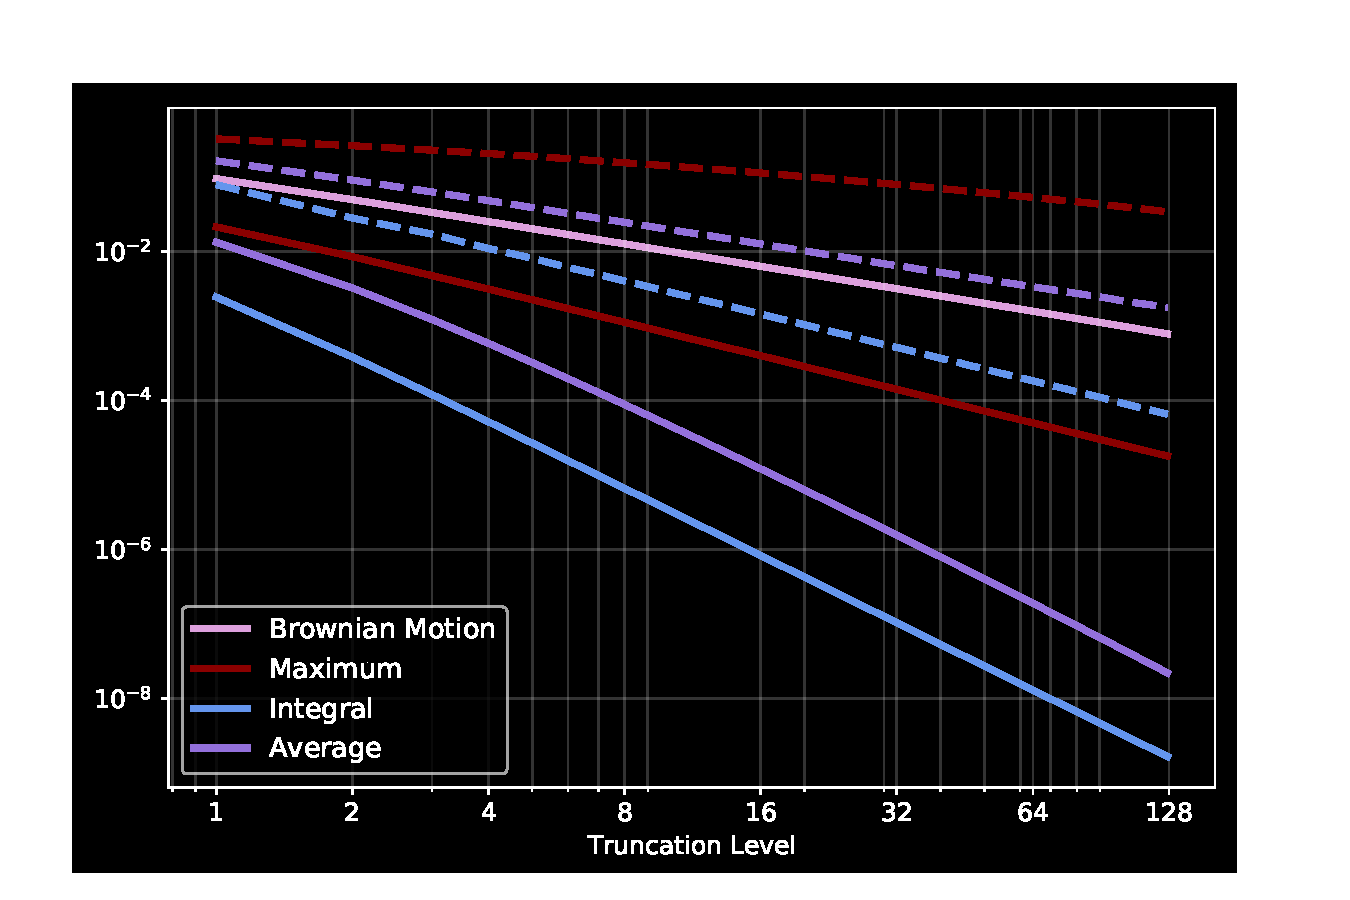
\includegraphics[scale =0.38]{KL/Figures/Error_nSim5000_N1000.pdf}
    \label{fig:L2Error}
    \\
    
    \vspace{1mm}
    
    \footnotesize{
    \textit{Dashed lines: functionals of projected paths. \\Solid lines: projected functionals.}}
\end{figure}

% \subsection{Monotone Convergence}
% When do we have $f_K \nearrow f$? This would ensure, in particular, that 
% $$\lim_{K\to \infty} \E^{\Q}[f_K(X_T)] = \E^{\Q}[f(X_T)].$$ 

% \begin{example}
% (\textbf{Running maximum}) Take 
% $f_K = f \circ \pi^{K,\frakF}$, where $\frakF$ are the Schauder functions and $\calH = \calR$. Then increasing the order $K$ adds new vertices on the graph of $x^{K,F}$ while keeping the ones already there. Hence the maximum, attained on a vertex can only increase. In other words, 
% $$f_K(X_t) = \max_{s\, \le t} x_s^{K,\frakF} = \max_{t_n\, \in \, \Pi_K} x_{t_n}^{K,\frakF} \le \max_{t_n\, \in \, \Pi_{K'}} x_{t_n}^{K',\frakF} = f_{K'}(X_t),
% $$
% if $\Pi_K$ denotes the $K-$th dyadic partition. 

% \end{example}



\subsection{Discussion: Projection of Functionals using the Signature} \label{sec:sigFunc}

Another approximation of $Y=f(X)$ can be obtained by combining  signature functionals in a linear fashion. For instance, one can consider all the words of length less than $\bar{K} \in \N$, giving the approximation
  \begin{equation}\label{eq:sigPayoff}
      y^{K,\calS}_t := \sum_{l(\alpha)\, \le \, \bar{K}} \xi^f_{\alpha} \calS_{\alpha}(X_t), 
  \end{equation}
  \vspace{-3mm}
  
  with $K = |\{\alpha \, | \, l(\alpha)\le \bar{K}\}|=2^{\bar{K}+1}-1.$
  The coefficients $\xi^f_{\alpha}$ may depend on  $X_0$  only and can be  calculated by either regressing  $Y$ against the signature elements or using a Taylor formula for functionals; see \cref{chap:Taylor}.  %\cite{LittererOberhauser} when $f$ is smooth (in the Dupire sense) and $X$ is a diffusion. 
    % In the literature,   $\eqref{eq:sigPayoff}$ is referred to  as  \textit{polynomial functional}  \cite{LittererOberhauser} or \textit{signature payoff} \cite{Szpruch,LyonsNum} in finance. 
     
     The appeal of such projection comes from the fact that polynomial functionals are dense in the space of continuous functionals restricted to  paths of bounded variation; see Theorem 5 in  \cite{LittererOberhauser}.  
     On the other hand, despite the existence of   packages to calculate the signature of discrete time paths (e.g., \texttt{iisignature} and \texttt{esig} in Python), the projection in $\eqref{eq:sigPayoff}$ is still  challenging from a computational perspective. 
     Indeed, contrary to the reconstruction in  \Cref{sec:sigLegendre}, the signature functionals have to be known at \textit{every} intermediate time. Also, as there is a priori no recipe to select words up to a given length,  we must retain all of them so the number of elements doubles every time a layer is added. 
